\documentclass[floatsintext,man]{apa6}

\usepackage{amssymb,amsmath}
\usepackage{ifxetex,ifluatex}
\usepackage{fixltx2e} % provides \textsubscript
\ifnum 0\ifxetex 1\fi\ifluatex 1\fi=0 % if pdftex
  \usepackage[T1]{fontenc}
  \usepackage[utf8]{inputenc}
\else % if luatex or xelatex
  \ifxetex
    \usepackage{mathspec}
    \usepackage{xltxtra,xunicode}
  \else
    \usepackage{fontspec}
  \fi
  \defaultfontfeatures{Mapping=tex-text,Scale=MatchLowercase}
  \newcommand{\euro}{€}
\fi
% use upquote if available, for straight quotes in verbatim environments
\IfFileExists{upquote.sty}{\usepackage{upquote}}{}
% use microtype if available
\IfFileExists{microtype.sty}{\usepackage{microtype}}{}

% Table formatting
\usepackage{longtable, booktabs}
\usepackage{lscape}
% \usepackage[counterclockwise]{rotating}   % Landscape page setup for large tables
\usepackage{multirow}		% Table styling
\usepackage{tabularx}		% Control Column width
\usepackage[flushleft]{threeparttable}	% Allows for three part tables with a specified notes section
\usepackage{threeparttablex}            % Lets threeparttable work with longtable

% Create new environments so endfloat can handle them
% \newenvironment{ltable}
%   {\begin{landscape}\begin{center}\begin{threeparttable}}
%   {\end{threeparttable}\end{center}\end{landscape}}

\newenvironment{lltable}
  {\begin{landscape}\begin{center}\begin{ThreePartTable}}
  {\end{ThreePartTable}\end{center}\end{landscape}}




% The following enables adjusting longtable caption width to table width
% Solution found at http://golatex.de/longtable-mit-caption-so-breit-wie-die-tabelle-t15767.html
\makeatletter
\newcommand\LastLTentrywidth{1em}
\newlength\longtablewidth
\setlength{\longtablewidth}{1in}
\newcommand\getlongtablewidth{%
 \begingroup
  \ifcsname LT@\roman{LT@tables}\endcsname
  \global\longtablewidth=0pt
  \renewcommand\LT@entry[2]{\global\advance\longtablewidth by ##2\relax\gdef\LastLTentrywidth{##2}}%
  \@nameuse{LT@\roman{LT@tables}}%
  \fi
\endgroup}


  \usepackage{graphicx}
  \makeatletter
  \def\maxwidth{\ifdim\Gin@nat@width>\linewidth\linewidth\else\Gin@nat@width\fi}
  \def\maxheight{\ifdim\Gin@nat@height>\textheight\textheight\else\Gin@nat@height\fi}
  \makeatother
  % Scale images if necessary, so that they will not overflow the page
  % margins by default, and it is still possible to overwrite the defaults
  % using explicit options in \includegraphics[width, height, ...]{}
  \setkeys{Gin}{width=\maxwidth,height=\maxheight,keepaspectratio}
\ifxetex
  \usepackage[setpagesize=false, % page size defined by xetex
              unicode=false, % unicode breaks when used with xetex
              xetex]{hyperref}
\else
  \usepackage[unicode=true]{hyperref}
\fi
\hypersetup{breaklinks=true,
            pdfauthor={},
            pdftitle={Polite speech emerges from competing pressures to be (and look) informative and kind},
            colorlinks=true,
            citecolor=blue,
            urlcolor=blue,
            linkcolor=black,
            pdfborder={0 0 0}}
\urlstyle{same}  % don't use monospace font for urls

\setlength{\parindent}{0pt}
%\setlength{\parskip}{0pt plus 0pt minus 0pt}

\setlength{\emergencystretch}{3em}  % prevent overfull lines


% Manuscript styling
\captionsetup{font=singlespacing,justification=justified}
\usepackage{csquotes}
\usepackage{upgreek}

 % Line numbering
  \usepackage{lineno}
  \linenumbers


\usepackage{tikz} % Variable definition to generate author note

% fix for \tightlist problem in pandoc 1.14
\providecommand{\tightlist}{%
  \setlength{\itemsep}{0pt}\setlength{\parskip}{0pt}}

% Essential manuscript parts
  \title{Polite speech emerges from competing pressures to be (and look)
informative and kind}

  \shorttitle{Modeling polite speech}


  \author{Erica J. Yoon\textsuperscript{1,F}, Michael Henry Tessler\textsuperscript{1,F}, Noah D. Goodman\textsuperscript{1}, \& Michael C. Frank\textsuperscript{1}}

  % \def\affdep{{"", "", "", ""}}%
  % \def\affcity{{"", "", "", ""}}%

  \affiliation{
    \vspace{0.5cm}
          \textsuperscript{1} Department of Psychology, Stanford University\\
          \textsuperscript{F} These authors contributed equally to this work.  }

  \authornote{
    FIXME.
    
    Correspondence concerning this article should be addressed to Erica J.
    Yoon, 450 Serra Mall, Bldg. 420, Rm. 290, Stanford, CA 94305. E-mail:
    \href{mailto:ejyoon@stanford.edu}{\nolinkurl{ejyoon@stanford.edu}}
  }


  \abstract{Conveying information in a false or indirect manner in consideration of
listeners' wants (i.e.~being polite) seemingly contradicts an important
goal of a cooperative speaker: information transfer. We model production
of polite speech in which speakers deviate from being maximally
informative for social reasons. In this work, we show that polite speech
emerges from a set of competing goals: to be informative, to be kind and
provide positive value to others, and to be self-presentational and
\emph{appear} helpful. We formalize this tradeoff between speaker's
competing goals using a utility-theoretic model, and show the model is
able to predict people's polite speech production judgments. Our
extension of formal theories of language to account for speakers' social
goals represents an advance in understanding of human speech.}
  \keywords{keywords \\

    \indent Word count: X
  }





\usepackage{amsthm}
\newtheorem{theorem}{Theorem}
\newtheorem{lemma}{Lemma}
\theoremstyle{definition}
\newtheorem{definition}{Definition}
\newtheorem{corollary}{Corollary}
\newtheorem{proposition}{Proposition}
\theoremstyle{definition}
\newtheorem{example}{Example}
\theoremstyle{definition}
\newtheorem{exercise}{Exercise}
\theoremstyle{remark}
\newtheorem*{remark}{Remark}
\newtheorem*{solution}{Solution}
\begin{document}

\maketitle

\setcounter{secnumdepth}{0}



We don't always say what is on our mind. Although \enquote{close the
window!} would be sufficient, we say \enquote{can you please \ldots{} ?}
or \enquote{would you mind \ldots{} ?} And rather than telling the
uncomfortable truth, we lie (\enquote{Your dress looks great!}) and
prevaricate (\enquote{your poem was so\ldots{} appropriate to the
occasion}). These kinds of utterances are puzzling for standard views of
language use, which see communication as the transfer of information
from a sender to a receiver (Bühler, 1934; M. C. Frank \& Goodman, 2012;
Jakobson, 1960; Shannon, 1948). Under information-based views, the
transfer ought to be efficient and accurate: The speaker should choose a
succinct utterance from which the listener can recover their intended
meaning (Grice, 1975; Searle, 1975), and the information transferred
should be accurate and truthful to the extent that the speaker knows or
believes to be true. Polite speech -- like the examples above -- then
violates basic expectations about the nature of communication: it is
typically inefficient and underinformative, and sometimes even outright
false. So why are we polite?

Theories of politeness explain deviations from optimal information
transfer in language by assuming that speakers take into account social,
as well as informational, concerns. These concerns are sometimes
expressed as sets of polite maxims (Leech, 1983) or social norms (Ide,
1989), but the most influential account of politeness relies on the
notion of \enquote{face} to motivate deviations (Brown \& Levinson,
1987; Goffman, 1967). On this theory, speakers seek to maintain both
their and the listeners' freedom to act (\enquote{negative face}) as
well as desires to be liked, approved, and related to (\enquote{positive
face}). Both inefficient indirect speech and untruthful lies in
communication are then due to speakers' strategic choices relative to
possible face threats.

This face-based framework provides an intuitive and appealing
explanation of many types of polite speech, but applying it to make
quantitative predictions in any individual circumstance can be
complicated. It is often not obvious how to quantify a face threat in a
given situation (e.g., how much of the listener's positive face will be
damaged by hearing \enquote{your poem was terrible}), or how social and
informational motivations will trade off in the mind of a speaker (given
that the poem recital was terrible, should the speaker say that the
listener's poem was \enquote{okay,} \enquote{not bad,} or
\enquote{marvelous}?). Concretely, such theorizing does not constrain
how an artificial agent like a robot should go about making polite
requests, conveying negative evaluations, or delivering bad news.
Further, it does not take into account the recursive nature of reasoning
about face: Speakers may choose particular strategies not only to
preserve face genuinely, but also to be \emph{seen} as doing so, hence
appearing to be considerate and socially apt.

To address these challenges, we develop a utility-theoretic model for
understanding polite speech, in a unified framework to quantify
tradeoffs between different goals that a speaker may have. In our model,
speakers attempt to maximize a set of competing utilities: an
informational utility, derived via effective information transmission; a
social utility, derived by being kind and providing positive affect to
others; and a self-presentational utility, derived by appearing in a
particular way to other agents. Speakers then can choose between
different utterances on the basis of their expected utility (including
their cost to utter, approximated by the length of the utterance). The
lie that a poem \enquote{was good} provides social utility by making its
writer feel good, but does not inform about the true state of the world.
Further, if the writer suspects that it was in fact terrible, the
speaker runs the risk of being seen as uncooperative.

Formally, these utilities are weighed within a rational speech act (RSA)
model. RSA models take a probabilistic approach to pragmatic reasoning
in language (M. C. Frank \& Goodman, 2012; Goodman \& Frank, 2016):
Speakers are modeled as agents who choose utterances by reasoning about
their effects on a listener relative to their cost, while listeners are
modeled as choosing interpretations by reasoning about speakers and
their goals. This class of models has been effective in understanding a
wide variety of complex linguistic behaviors, including vagueness
(Lassiter \& Goodman, 2017), hyperbole (Kao, Wu, Bergen, \& Goodman,
2014), and irony (Kao \& Goodman, 2015), among others. More broadly, RSA
models provide a instantiation for language of the idea that human
social cognition can be approximated via reasoning about others as
rational agents who act to maximize their subjective utility (Baker,
Saxe, \& Tenenbaum, 2009), a hypothesis which has found support in a
wide variety of work with both adults and children (e.g., Jara-Ettinger,
Gweon, Schulz, \& Tenenbaum, 2016; Liu, Ullman, Tenenbaum, \& Spelke,
2017).

\begin{figure}
\centering
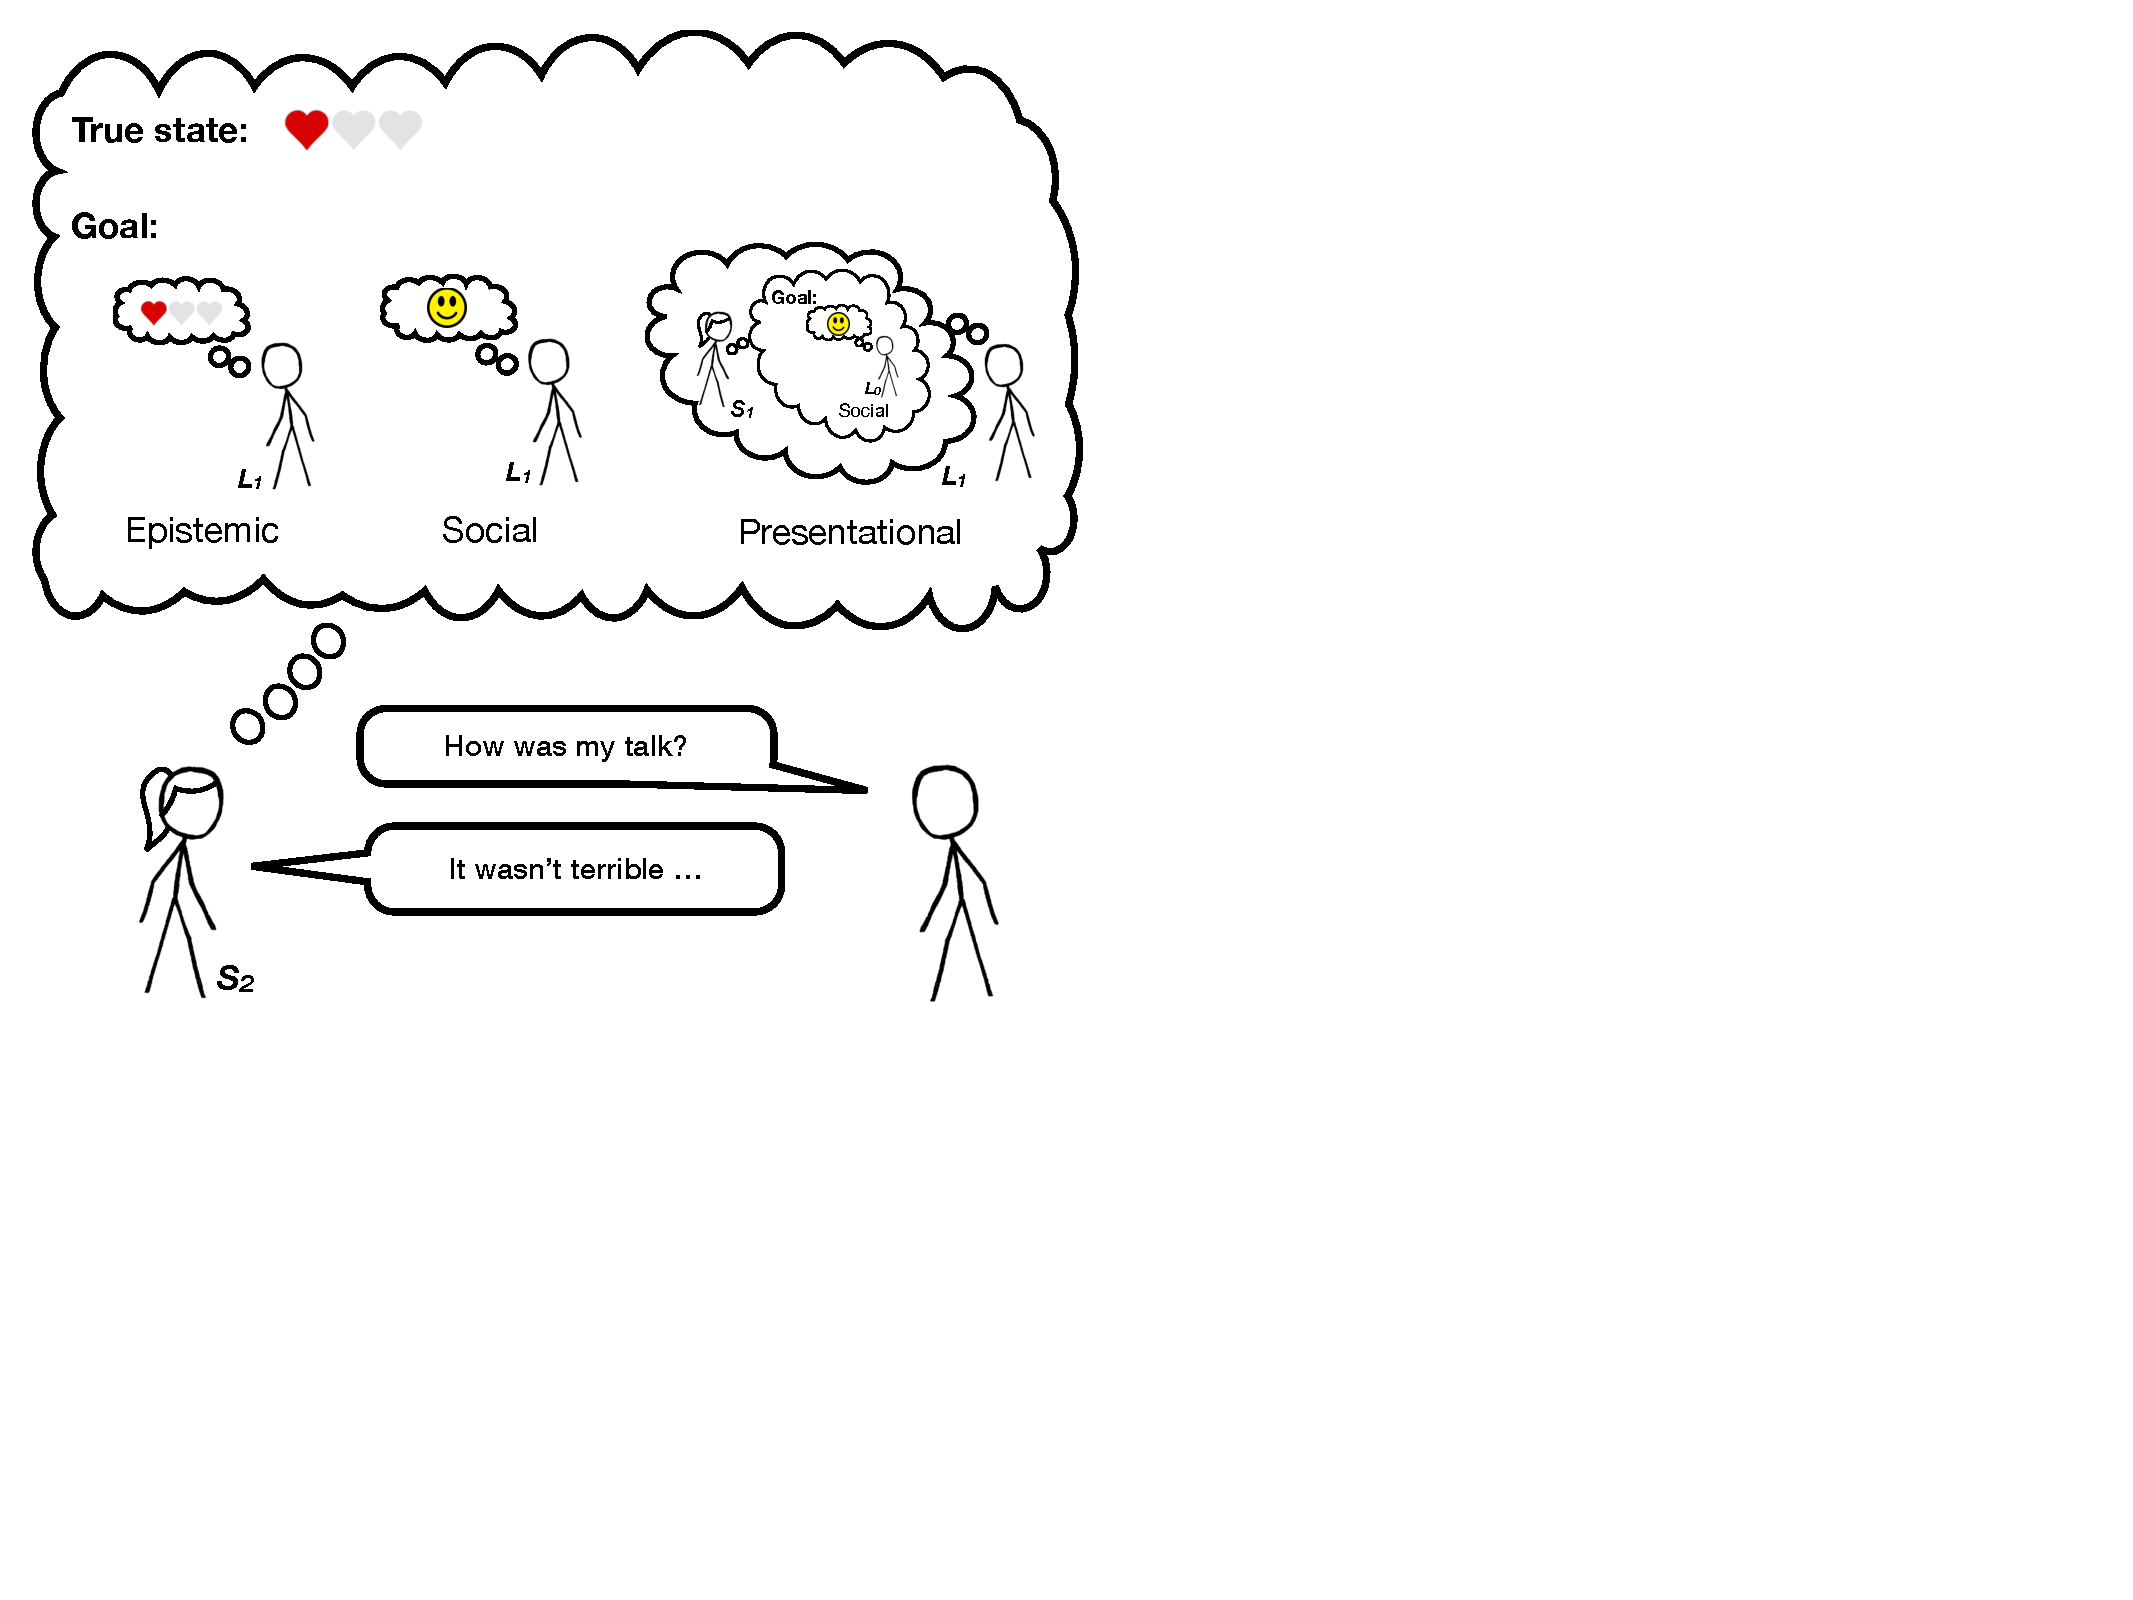
\includegraphics{fig/model.pdf}
\caption{\label{fig:model}Diagram of the model: The pragmatic speaker
observes the true state and determines her goal between three utilities
(epistemic, social, and presentational), and produces an utterance.}
\end{figure}

RSA models are defined recursively such that speakers reason about
listeners, and vice versa. By convention the level of this recursion is
numbered such that a pragmatic listener \(L_1\) reasons about what
intended meaning and goals would have led a speaker \(S_1\) to produce a
particular utterance. Then S1 reasons about a \enquote{literal listener}
\(L_0\), who is modeled as attending only to the literal meanings of
words (rather than their pragmatic implications), and hence grounds the
recursion. The target of our current work is a model of a polite speaker
\(S_2\): \(S_2\) reasons about what utterance to say to \(L_1\) by
considering the set of utilities described above: namely, whether an
utterance results in \(L_1\) gaining information, feeling positively, or
judging \(S_2\) to be either informative or kind (Figure
\ref{fig:model}).

We evaluate our model by predicting human behavioral data in situations
where polite language use is expected. Imagine Bob recited his poem and
is ignorant of the quality of his poem recital; he asks Ann how well he
did. Ann (the pragmatic speaker \(S_2\)) produces an utterance \(w\)
based on the true state of the world \(s\) (i.e., the rating truly
deserved by Bob's recital) and a set of goal weights \(\hat{\phi}\),
each of which determines how much she would like to prioritize a
particular goal compared to other possible goals. The speaker chooses
utterances depending on their expected utility, specifically as a
softmax which interpolates between maximizing and matching (via the
parameter \(\lambda_{S_2}\); Goodman \& Stuhlmüller, 2013):

\[P_{S_2}(w | s, \hat{\phi}) \propto \exp(\lambda_{S_2} \cdot \mathop{\mathbb{E}}[U_{total}(w; s; \hat{\phi})])\].

What goals must the speaker consider to arrive at a polite utterance? We
consider three utilities: informational, social, and presentational. The
total utility of an utterance is the weighted combination of the three
utilities minus the cost \(C(w)\):

\[U_{total}(w; s; \hat{\phi}) = \phi_{inf} \cdot U_{inf}(w; s) + \phi_{soc} \cdot U_{soc}(w; s) + \phi_{pres} \cdot U_{pres}(w; s) - C(w)\].

The first utility term is a standard \emph{informational utility}
(\(U_{inf}\)), which represents the speaker's desire to be epistemically
helpful. The informational utility captures the amount of information a
literal listener (\(L_0\)) would still not know about the world state
after hearing the speaker's utterance:

\[U_{inf}(w) = \ln(P_{L_1}(s | w))\].

For aspects of the world with affective consequences for the listener
(e.g., Bob and his poem recital), we assume speakers produce utterances
that make listeners feel like they are in a good state. \emph{Social
utility} (\(U_{soc}\)) is the value, or expected subjective utility, to
the listener of the state inferred given the utterance. This value
captures the idea that people want to hear that they are in a good state
of the world (e.g., that Bob's poem recital was good). We use a simple
linear value function (\(V\)) to map states to subjective values: better
ratings are more positively valued:

\[U_{soc}(w) = \mathbb{E}_{P_{L_1}(s \mid w)}[V(s)]\].

If listeners are aware that speakers have goals and try to infer what
those goals are, speakers may choose utterances in order to convey that
they had certain goals in mind. The third component,
\emph{presentational utility} (\(U_{pres}\)), captures the extent to
which the speaker appears to the listener to have a particular goal in
mind (e.g.~to be kind). The speaker gains presentational utility when
her listener believes she has certain goals -- that she is trying to be
informative or kind. Formally,

\[U_{pres}(w) = \ln(P_{L_1}(\phi_{S_1} \mid w)) = \ln \int_s P_{L_1}(s, \phi_{S_1} \mid w)\].

The speaker considers the beliefs of listener L1, who hears an utterance
and jointly infers both the speaker's utilities and the true state of
the world:

\[P_{L_1}(s, \hat{\phi} | w) \propto P_{S_1}(w | s, \hat{\phi}) \cdot P(s) \cdot p(\hat{\phi})\].

This presentational utility, which is the most novel aspect of our
model, is higher-order in that it can only be defined for a speaker
thinking about a listener who evaluates a speaker. (That is, it can be
defined for \(S_2\), but not \(S_1\).)

Finally, utterances that are more complex incur a greater cost, \(C(w)\)
-- capturing the general pressure towards economy in speech. In our
work, utterances with negation (e.g., \enquote{not terrible}) are
slightly more costly than their equivalents with no negation (inferred
from data; see Supplemental Materials).

Intuitively, when Bob's performance is good, Ann's utilities align to
lead her to say something positive. By saying \enquote{{[}Your poem
recital{]} was amazing,} Ann is being both truthful and kind, and that
is likely to be clear to Bob. But, if Bob's recital is poor, Ann is in a
bind: She could be kind and say it was great, but she does so at the
cost of conveying the wrong information to Bob, if he mistakenly infers
Ann's goal to be truthful and his recital to be actually good. Worse
yet, Bob could infer that she is \enquote{just being nice,} inferring
her goal to be social, and discount her comment as uninformative.
Alternatively, she could directly say the truth (\enquote{It was bad}),
but then Bob would think Ann didn't care about him. What is a
socially-aware speaker to do? Our model predicts that indirect speech --
like \enquote{It wasn't bad} -- helps navigate Ann's dilemma. It conveys
some true information while being sufficiently open-ended to spare Bob's
feelings. Further, by incurring the slightly higher cost involved in
producing another word suggests that Ann had reasons for not saying a
simpler alternative like \enquote{It was good,} and thus it provides a
signal to Bob that Ann takes his feelings into account in her choice.

We made a direct, pre-registered test of our model by instantiating the
example above in an online experiment (\emph{N} = 202). Participants
read scenarios in which we provided information on the speaker's (Ann's,
in our example) feelings toward some performance or product (e.g., poem
recital; \emph{true state}), which were shown on a scale from zero to
three hearts (e.g.~one out of three hearts). For example, one trial
read: \enquote{Imagine that Bob gave a poem recital, but he didn't know
how good it was. Bob approached Ann, who knows a lot about poems, and
asked}How was my poem?" We also manipulated the speaker's \emph{goal}
across trials: to be \emph{informative} and \enquote{give accurate and
informative feedback}; to be \emph{social} and \enquote{to make the
listener feel good}; or to be \emph{both} informative and social at the
same time. We hypothesized that each of the three goals will represent a
tradeoff between the three utilities in our model described above (their
inferred values are available in the Supplementary Materials). In a
single trial, each scenario was followed by a question that asked for
the most likely utterance by Ann. Participants selected one of eight
possible utterances, by choosing between \emph{It was} vs. \emph{It
wasn't} and then among \emph{terrible}, \emph{bad}, \emph{good}, and
\emph{amazing.}

\begin{figure}
\centering
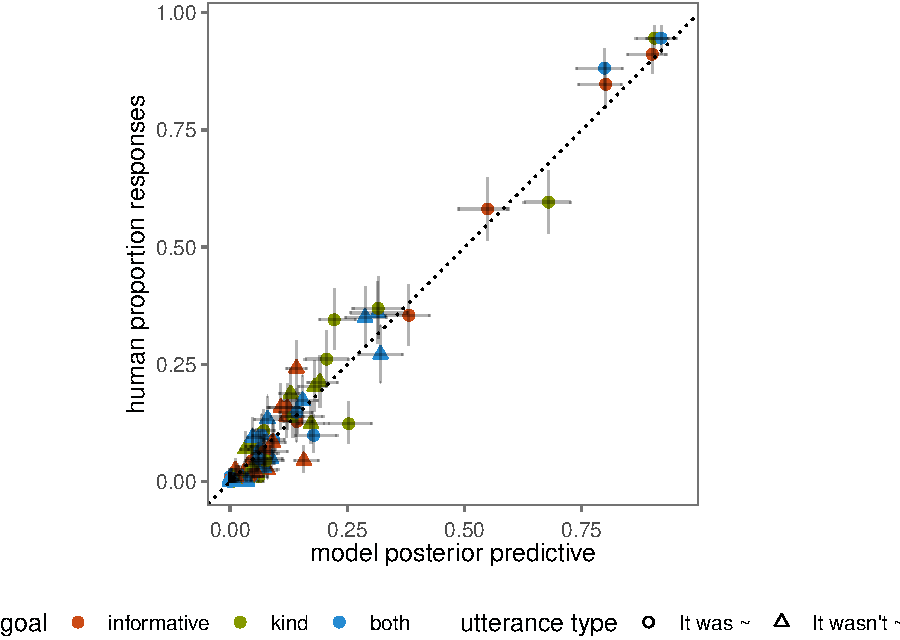
\includegraphics{polite_manuscript_files/figure-latex/variance-1.pdf}
\caption{\label{fig:variance}Full distribution of human responses vs.~model
predictions. Error bars represent 95\% confidence intervals for the data
(vertical) and 95\% highest density intervals for the model
(horizontal).}
\end{figure}

Our primary behavioral hypothesis was that speakers who found themselves
describing bad states (e.g., Bob's performance was bad) and who had as
goals to be both informative and social would produce more indirect,
negative utterances (\enquote{It wasn't terrible}). These indirect
speech acts serve to save the listener's face while also conveying a
vague estimate of the true state. This prediction was confirmed: a
Bayesian mixed-effects model predicting negation as a function of true
state and goal yielded a significant interaction, such that a speaker
with both informational and social goals produced more negation in worse
states compared to a speaker with only the informational goal (\emph{M}
= -1.33, {[}-1.69, -0.98{]}) and social goal (\emph{M} = -0.50,
{[}-0.92, -0.07{]}). Rather than eschewing one of their goals to
increase utility along a single dimension, participants chose utterances
that jointly satisfied their conflicting goals by producing indirect,
polite speech.

To connect these behavioral data more directly to our model, we next
built a Bayesian data analytic model to integrate out the parameters of
the RSA model (e.g., the condition-specific goal-weights for the
speaker) and provide a principled way to incorporate judgments about the
literal meanings of the utterances into our model's predictions {[}Lee
and Wagenmakers (2014); see Supplementary Materials{]}. Using an
independent sample of N=51 participants, we measured how participants
judged our possible utterances to apply to each of the levels on the
heart scale (e.g., to what extent is \enquote{terrible} true of 2 out of
3 hearts?). These measurements are used in the Bayesian data analysis to
approximate the semantics of the words as interpreted by the literal
listener agent L0 (see Supplementary Materials for literal semantic
results; see our pre-registered model, hypothesis, and procedure at
FIXME).

\begin{figure}
\centering
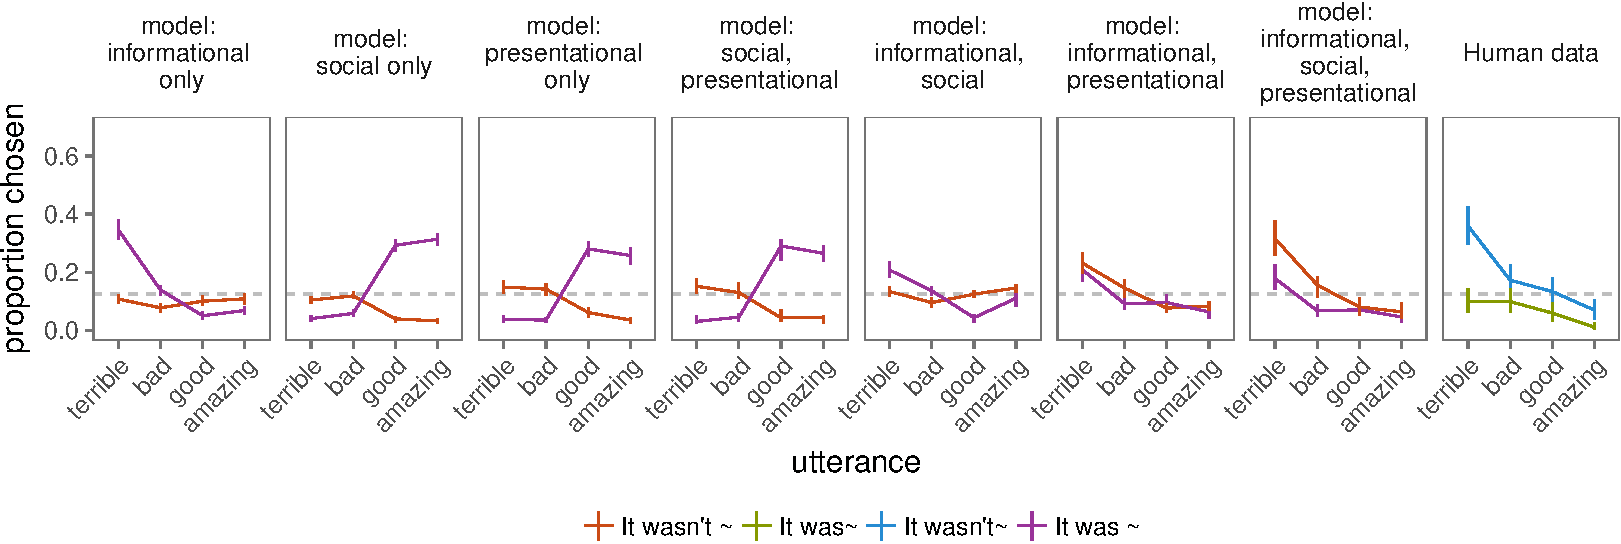
\includegraphics{polite_manuscript_files/figure-latex/comparison-1.pdf}
\caption{\label{fig:comparison}Comparison of predictions for proportion of
utterances chosen by pragmatic speaker from possible model variants
(left) and human data (rightmost) for average proportion of negation
produced among all utterances, given true state of 0 heart (on a scale
of 0 to 3) and speaker with both goals. Gray dotted line indicates
chance level at 12.5\%.}
\end{figure}

\begin{table}[tbp]
\begin{center}
\begin{threeparttable}
\caption{\label{tab:comparisonTable}Comparison of variance explained for each model variant and log Bayes factors (with the marginal likelihood for the full model as the denominator).
}
\begin{tabular}{lll}
\toprule
Model & \multicolumn{1}{c}{Variance 
explained} & \multicolumn{1}{c}{log BF}\\
\midrule
model: 
informative only & 0.83 & 274.89\\
model: 
social only & 0.22 & 885.52\\
model: 
presentational 
only & 0.23 & 873.83\\
model: 
social, 
presentational & 0.23 & 864.00\\
model: 
informative, 
social & 0.92 & 25.06\\
model: 
informative, 
presentational & 0.96 & 11.14\\
model: 
informative, 
social, 
presentational & 0.97 & 1.00\\
\bottomrule
\end{tabular}
\end{threeparttable}
\end{center}
\end{table}

Predictions from the full polite speaker model showed a strong fit to
participants' utterance choices (\(r^2\)(96) = 0.97; Figure
\ref{fig:variance}). We also compared the predictions of our model with
model variants containing different subsets of the three utilities in
the full model (Figure 3; see Supplemental Materials: Model Comparison).
Both the variance explained and the likelihood were the highest for the
full model (see Table \ref{tab:comparisonTable} and Figure
\ref{fig:comparison}). In particular, only the full model captured the
participants' preference for negation in the condition in which the
speaker had both goals to be informative and social about truly bad
states, as we hypothesized. The full model was superior to: the model
with social and presentational utilities, which predicted outright false
statements (\enquote{It was good}); the model with informational and
social utilities, which predicted truthful statements \enquote{It was
terrible} and \enquote{It wasn't amazing} (that is semantically true
when the poem was terrible); and to the model with informative and
presentational utilities, which predicted that the speaker would now
care about being seen as informative and nice, but still wanting to be
as truthful (\enquote{It was terrible}) as she is presentational
(\enquote{It wasn't terrible}). Thus, all three -- informational,
social, and presentational -- utilities were required to fully explain
participants' choices, correctly predicting that they would prefer to
say an indirect speech (\enquote{It wasn't terrible}) about a bad
performance.

Politeness is a puzzle for purely informational accounts of language
use. Incorporating social motivations can provide an explanatory
framework, but such intuitions have been resistant to formalization or
precise testing. To overcome this issue, we created a utility-theoretic
model of language use that captured the interplay between competing
informational, social, and presentational goals. A preregistered
experimental test of the model confirmed its ability to capture human
judgments, unlike comparison models that used only a subset of the full
utility structure.

To better measure choice behavior, our experiment abstracted away from
natural interactions in a number of ways. Real-life Anns will have
access to a potentially infinite range of utterances to manage the same
tradeoff (\enquote{It's so hard to write a good poem,} \enquote{That
metaphor in the second stanza was so relatable!}). Under our framework,
each utterance will have strengths and weaknesses relative to the
speaker's goals, though computation in an unbounded model presents
technical challenges (see Goodman \& Frank, 2016).

Managing listeners' inferences is a fundamental task for a socially
conscious speaker. Following Brown and Levinson (1987) we hypothesize
that cross-cultural differences in politeness are a product of different
weightings within the same utility structure. Systematic measurements of
these weights could be an approach to understanding the vast range of
politeness practices found across languages. Further, politeness is only
one of the ways that language use deviates from pure information
transfer. When we flirt, insult, boast, and empathize, we balance
information transmission with the goal to affect others' feelings or
present particular views of ourselves. A similar utility structure to
the one we employed here could give insights into these behaviors as
well.

The formalization of the presentational utility is especially meaningful
in that it begins to precisely define self-oriented motivations behind
polite speech and other related behaviors. Brown and Levinson, and other
theories of politeness described that other- vs.~self-oriented
strategies are different (e.g., maximize approval of other, minimize
praise of self; Leech, 1983), but did not explain how the motivations of
the two are related or how they trade off to inform the speaker's
utterance choices. In our current model, the self-oriented concern stems
from an other-oriented concern, as the speaker wants to appear to care
about the other person's face or access to knowledge. The model then
makes precise predictions about how the speaker considering both of
these concerns will choose her utterances. This work then can be
extended to not only other speech acts, but also a wide range of
behaviors that can be modeled as utility-driven inference in a social
context (Baker, Jara-Ettinger, Saxe, \& Tenenbaum, 2017; Hamlin, Ullman,
Tenenbaum, Goodman, \& Baker, 2013) where agents need to take into
account concerns about both self and others.

In sum, this work takes a concrete step toward quantitative models of
the nuances of human speech. And it moves us closer to courteous
computation -- to computers that communicate with tact.

\section{Acknowledgments}\label{acknowledgments}

This work was supported by NSERC PGS Doctoral scholarship
PGSD3-454094-2014 to EJY, NSF Graduate Research Fellowship DGE-114747 to
MHT, ONR grant N00014-13-1-0788 to NDG, and NSF grant BCS 1456077 to
MCF.

\newpage

\section{Supplemental Materials}\label{supplemental-materials}

\subsection{Materials and Methods}\label{materials-and-methods}

\subsubsection{Literal semantic task}\label{literal-semantic-task}

We probed judgments of literal meanings of the target words assumed by
our model and used in all our experiments. 51 participants with IP
addresses in the United States were recruited on Amazon's Mechanical
Turk. We used 13 different context items in which someone evaluated a
performance of some kind. For example, in one of the contexts, Ann saw a
presentation, and Ann's feelings toward the presentation (true state)
were shown on a scale from zero to three hearts (e.g., two out of three
hearts filled in red color). The question of interest was ''Do you think
Ann thought the presentation was / wasn't X?'' and participants
responded by choosing either \enquote{no} or \enquote{yes.} The target
could be one of five possible words: terrible, bad, good, and amazing,
giving rise to ten different possible utterances (with negation or no
negation). Each participant read 32 scenarios, depicting every possible
combination of states and utterances. The order of context items was
randomized, and there were a maximum of four repeats of each context
item per participant. For this and the subsequent experiment, we
analyzed the data by collapsing across context items. For each
utterance-state pair, we computed the posterior distribution over the
semantic weight (i.e., how consistent X utterance is with Y state)
assuming a uniform prior over the weight. Meanings of the words as
judged by participants were as one would expect (see Figure S1). We used
the fraction of participants that endorsed utterance w for state s to
set informative priors to infer posterior credible values of the literal
meanings from data in the speaker production experiment.

\subsubsection{Speaker production task}\label{speaker-production-task}

202 participants with IP addresses in the United States were recruited
on Amazon's Mechanical Turk. As in the literal semantic task above, we
used scenarios in which a person (e.g., Bob) gave some performance and
asked for another person (e.g., Ann)'s opinion on the performance (see
Fig. 2). Additionally, we provided information on the speaker Ann's goal
-- to make Bob feel good, or to give as accurate and informative
feedback as possible, or both -- and the true state -- how Ann actually
felt about Bob's performance (e.g., two out of three hearts, on a scale
from zero to three hearts). Each participant read 12 scenarios,
depicting every possible combination of goals (3) and states (4). The
order of context items was randomized, and there were a maximum of two
repeats of each context item per participant. Each scenario was followed
by a question that read, ''If Ann wanted to make Bob feel good but not
necessarily give informative feedback (or to give accurate and
informative feedback but not necessarily make Bob feel good, or BOTH
make Bob feel good AND give accurate and informative feedback), what
would Ann be most likely to say?'' Participants indicated their answer
by choosing one of the options on the two dropdown menus, side-by-side,
one for choosing between It was vs.~It wasn't and the other for choosing
among terrible, bad, good, and amazing.

\subsection{Supplementary Text}\label{supplementary-text}

\subsubsection{Data analysis}\label{data-analysis}

We used R (Version 3.4.3; R Core Team, 2017) and the R-packages
\emph{BayesFactor} (Version 0.9.12.2; Morey \& Rouder, 2015),
\emph{bindrcpp} (Version 0.2; Müller, 2017a), \emph{binom} (Version
1.1.1; Dorai-Raj, 2014), \emph{brms} (Version 2.0.1; Bürkner, 2017),
\emph{coda} (Version 0.19.1; Plummer, Best, Cowles, \& Vines, 2006),
\emph{directlabels} (Version 2017.3.31; Hocking, 2017), \emph{dplyr}
(Version 0.7.4; Wickham, Francois, Henry, \& Müller, 2017),
\emph{forcats} (Version 0.2.0; Wickham, 2017a), \emph{ggplot2} (Version
2.2.1; Wickham, 2009), \emph{ggthemes} (Version 3.4.0; Arnold, 2017),
\emph{gridExtra} (Version 2.3; Auguie, 2017), \emph{here} (Version 0.1;
Müller, 2017b), \emph{jsonlite} (Version 1.5; Ooms, 2014),
\emph{langcog} (Version 0.1.9001; Braginsky, Yurovsky, \& Frank, n.d.),
\emph{lme4} (Version 1.1.15; Bates, Mächler, Bolker, \& Walker, 2015),
\emph{magrittr} (Version 1.5; Bache \& Wickham, 2014), \emph{Matrix}
(Version 1.2.12; Bates \& Maechler, 2017), \emph{papaja} (Version
0.1.0.9655; Aust \& Barth, 2017), \emph{purrr} (Version 0.2.4; Henry \&
Wickham, 2017), \emph{RColorBrewer} (Version 1.1.2; Neuwirth, 2014),
\emph{Rcpp} (Eddelbuettel \& Balamuta, 2017; Version 0.12.14;
Eddelbuettel \& François, 2011), \emph{readr} (Version 1.1.1; Wickham,
Hester, \& Francois, 2017), \emph{rwebppl} (Version 0.1.97; Braginsky,
Tessler, \& Hawkins, n.d.), \emph{stringr} (Version 1.2.0; Wickham,
2017b), \emph{tibble} (Version 1.3.4; Müller \& Wickham, 2017),
\emph{tidyr} (Version 0.7.2; Wickham \& Henry, 2017), and
\emph{tidyverse} (Version 1.2.1; Wickham, 2017c) for all our analyses.

\subsubsection{Full statistics on human
data}\label{full-statistics-on-human-data}

\begin{table}[tbp]
\begin{center}
\begin{threeparttable}
\caption{\label{tab:brmTab}Predictor mean estimates with standard deviation and 95\% credible interval information for a Bayesian linear mixed-effects model predicting negation production based on true state and speaker goal (with both-goal as the reference level).}
\begin{tabular}{lllll}
\toprule
Predictor & \multicolumn{1}{c}{Mean} & \multicolumn{1}{c}{SD} & \multicolumn{1}{c}{95\% CI-Lower} & \multicolumn{1}{c}{95\% CI-Upper}\\
\midrule
Intercept & 0.88 & 0.13 & 0.63 & 1.12\\
True state & 2.18 & 0.17 & 1.86 & 2.53\\
Goal: Informative & 0.47 & 0.17 & 0.14 & 0.80\\
Goal: Social & 0.97 & 0.25 & 0.51 & 1.49\\
True state * Informative & -1.33 & 0.18 & -1.69 & -0.98\\
True state * Social & -0.50 & 0.22 & -0.92 & -0.07\\
\bottomrule
\end{tabular}
\end{threeparttable}
\end{center}
\end{table}

We used Bayesian linear mixed-effects models (\texttt{brms} package in
R; Bürkner, 2017) using crossed random effects of true state and goal
with maximal random effects structure ({\textbf{???}}, {\textbf{???}}).

\subsubsection{Model fitting and inferred
parameters}\label{model-fitting-and-inferred-parameters}

\begin{table}[tbp]
\begin{center}
\begin{threeparttable}
\caption{\label{tab:phi}Inferred phi parameters from all model variants with more than one utility.}
\begin{tabular}{llllll}
\toprule
Model & \multicolumn{1}{c}{goal} & \multicolumn{1}{c}{$\phi_{inf}$} & \multicolumn{1}{c}{$\phi_{soc}$} & \multicolumn{1}{c}{$\phi_{pres}$} & \multicolumn{1}{c}{$\phi_{S_1}$}\\
\midrule
informative, social, presentational & both & 0.36 & 0.11 & 0.54 & 0.36\\
informative, social, presentational & informative & 0.36 & 0.02 & 0.62 & 0.49\\
informative, social, presentational & social & 0.25 & 0.31 & 0.44 & 0.37\\
informative, presentational & both & 0.64 & NA & 0.36 & 0.17\\
informative, presentational & informative & 0.77 & NA & 0.23 & 0.33\\
informative, presentational & social & 0.66 & NA & 0.34 & 0.04\\
informative, social & both & 0.54 & 0.46 & NA & NA\\
informative, social & informative & 0.82 & 0.18 & NA & NA\\
informative, social & social & 0.39 & 0.61 & NA & NA\\
social, presentational & both & NA & 0.38 & 0.62 & 0.55\\
social, presentational & informative & NA & 0.35 & 0.65 & 0.75\\
social, presentational & social & NA & 0.48 & 0.52 & 0.66\\
\bottomrule
\end{tabular}
\end{threeparttable}
\end{center}
\end{table}

\begin{table}[tbp]
\begin{center}
\begin{threeparttable}
\caption{\label{tab:otherParams}Inferred negation cost and speaker optimality parameters for all model variants.}
\begin{tabular}{lll}
\toprule
Model & \multicolumn{1}{c}{Cost of negation} & \multicolumn{1}{c}{Speaker optimality}\\
\midrule
informative only & 1.58 & 8.58\\
informative, presentational & 1.89 & 2.93\\
informative, social & 1.11 & 3.07\\
informative, social, presentational & 2.64 & 4.47\\
presentational only & 2.58 & 9.58\\
social only & 1.73 & 7.23\\
social, presentational & 2.49 & 5.29\\
\bottomrule
\end{tabular}
\end{threeparttable}
\end{center}
\end{table}

In the speaker production task, participants were told what speakers'
intentions were (e.g., wanted to make Bob feel good). We assume that the
intention descriptions conveyed the weight mixtures \(\phi_{epi}\),
\(\phi_{soc}\), \(\phi_{pres}\), and \(\phi_{S_1}\) that the speaker was
using. We put uninformative priors on each of these mixtures (\(\phi\)
\textasciitilde{} \(Uniform(0,1)\)) and inferred their credible values
separately for each goal condition (\enquote{wanted to X}) using
Bayesian data analytic techniques (Lee \& Wagenmakers, 2014). We ran 4
MCMC chains for 80,000 iterations, discarding the first 40,000 for
burnin. The inferred values of weight mixtures for each model variant
(with different \(\phi\) components) and other parameters are shown in
Table \ref{tab:phi} and Table \ref{tab:otherParams} respectively.

\newpage

\subsection{Supplemental Figures}\label{supplemental-figures}

\begin{figure}[!h]
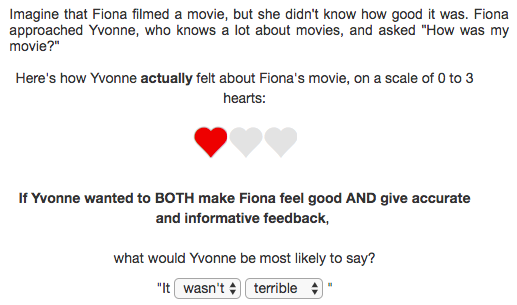
\includegraphics[width=3.98in]{fig/screenshot} \caption{Example of a trial in the speaker production task.}\label{fig:screenshot}
\end{figure}

\begin{figure}[!h]
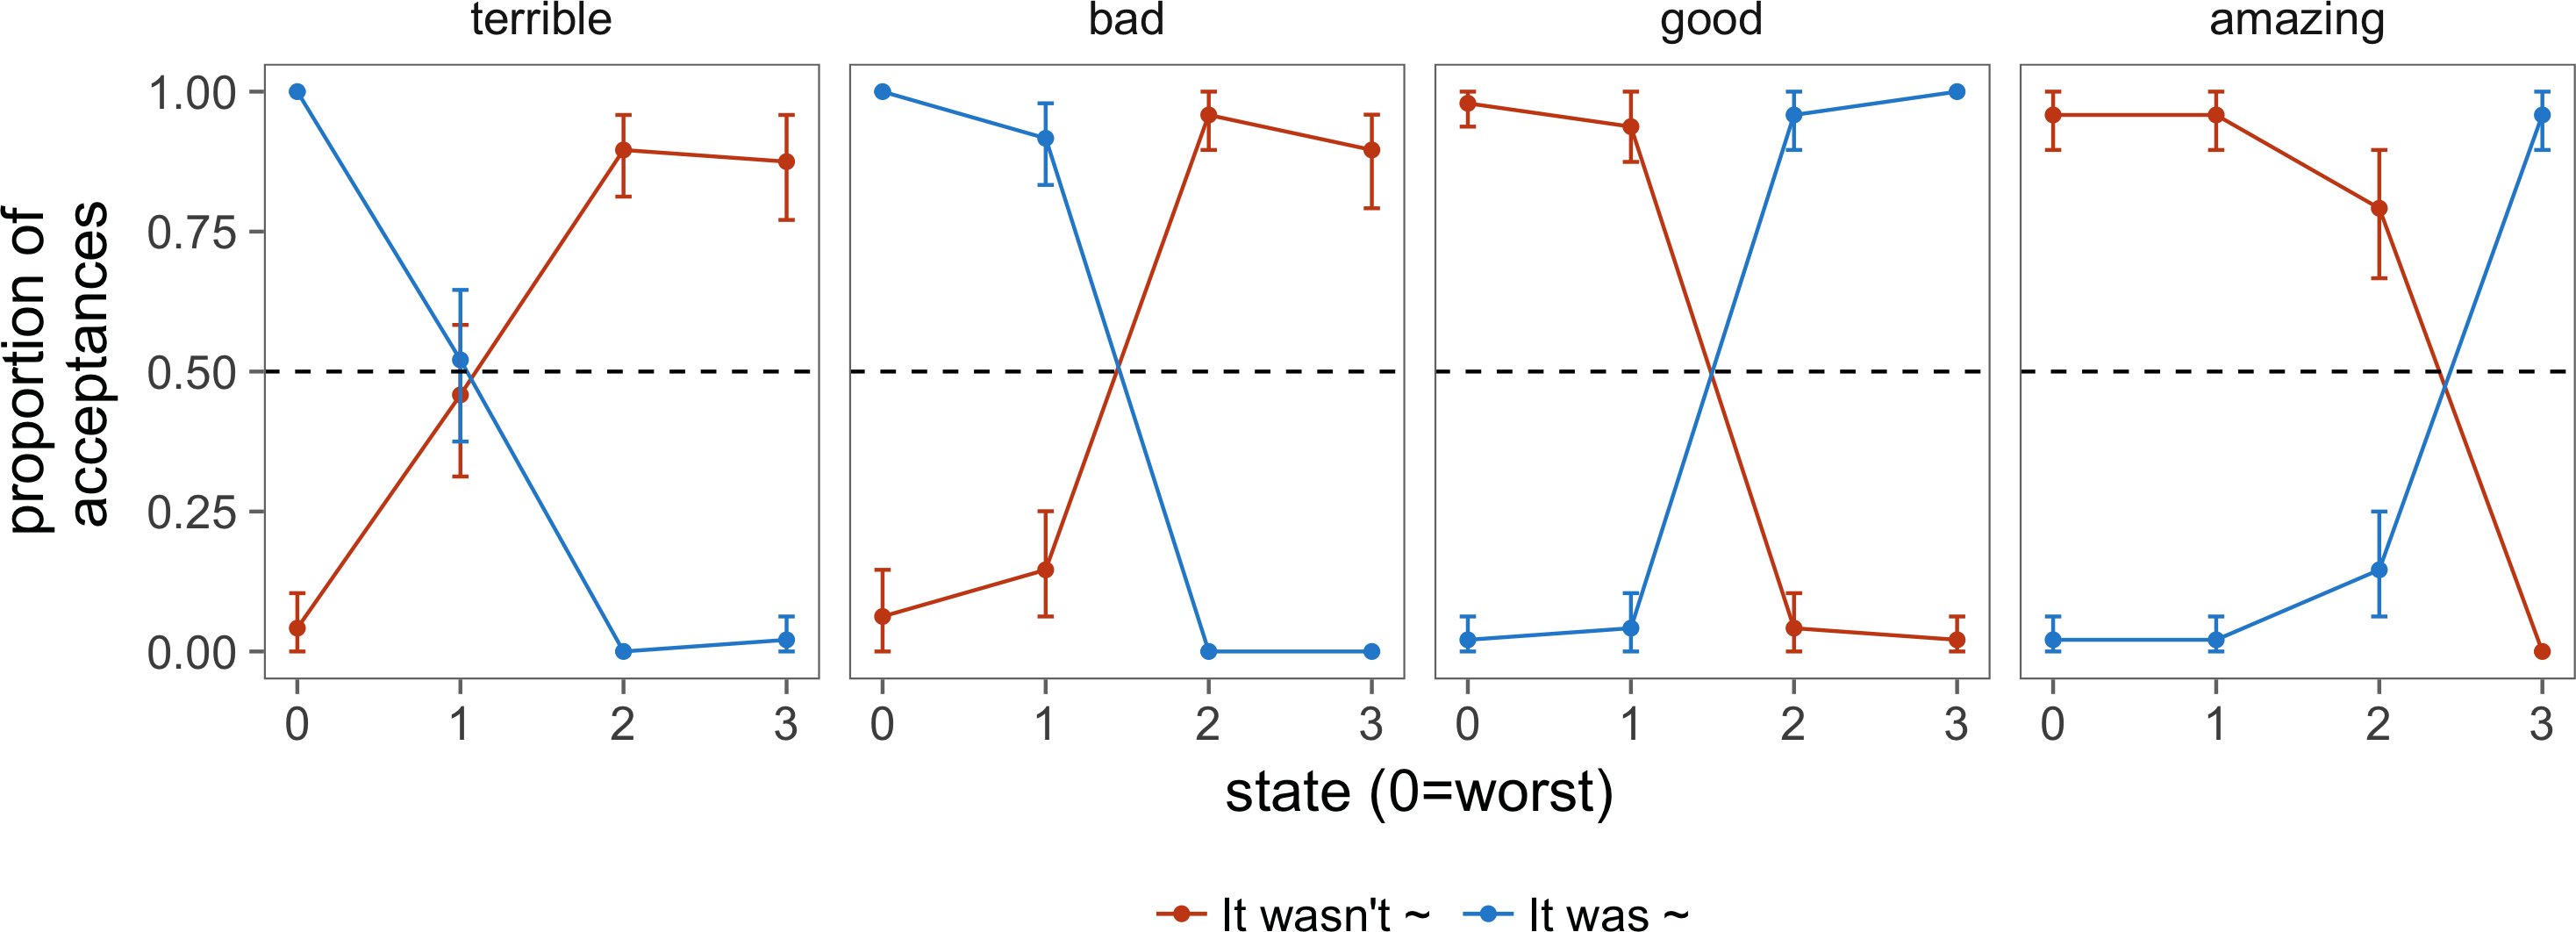
\includegraphics[width=\textwidth]{polite_manuscript_files/figure-latex/litsem-1} \caption{Semantic measurement results. Proportion of acceptances of utterance types (shown in different colors) combined with target words (shown in different facets) given the true state represented on a scale of hearts. Error bars represent 95\% confidence intervals.}\label{fig:litsem}
\end{figure}

\begin{figure}[!h]
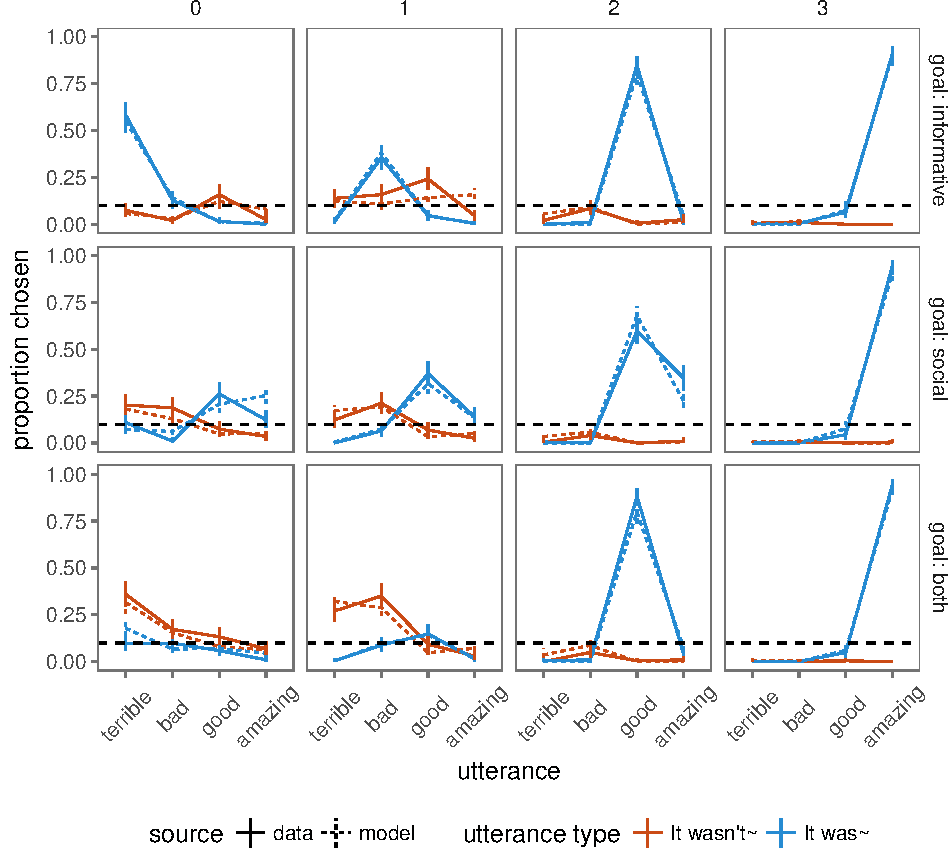
\includegraphics[width=\textwidth]{polite_manuscript_files/figure-latex/utterance-1} \caption{Experimental results (solid lines) and fitted predictions from the full model (dashed lines) for speaker production. Proportion of utterances chosen (utterance type – direct vs. indirect – in different colors and words shown on x-axis) given the true states (columns) and speaker goals (rows). Error bars represent 95\% confidence intervals for the data and 95\% highest density intervals for the model. Black dotted line represents the chance level.}\label{fig:utterance}
\end{figure}

\begin{figure}[!h]
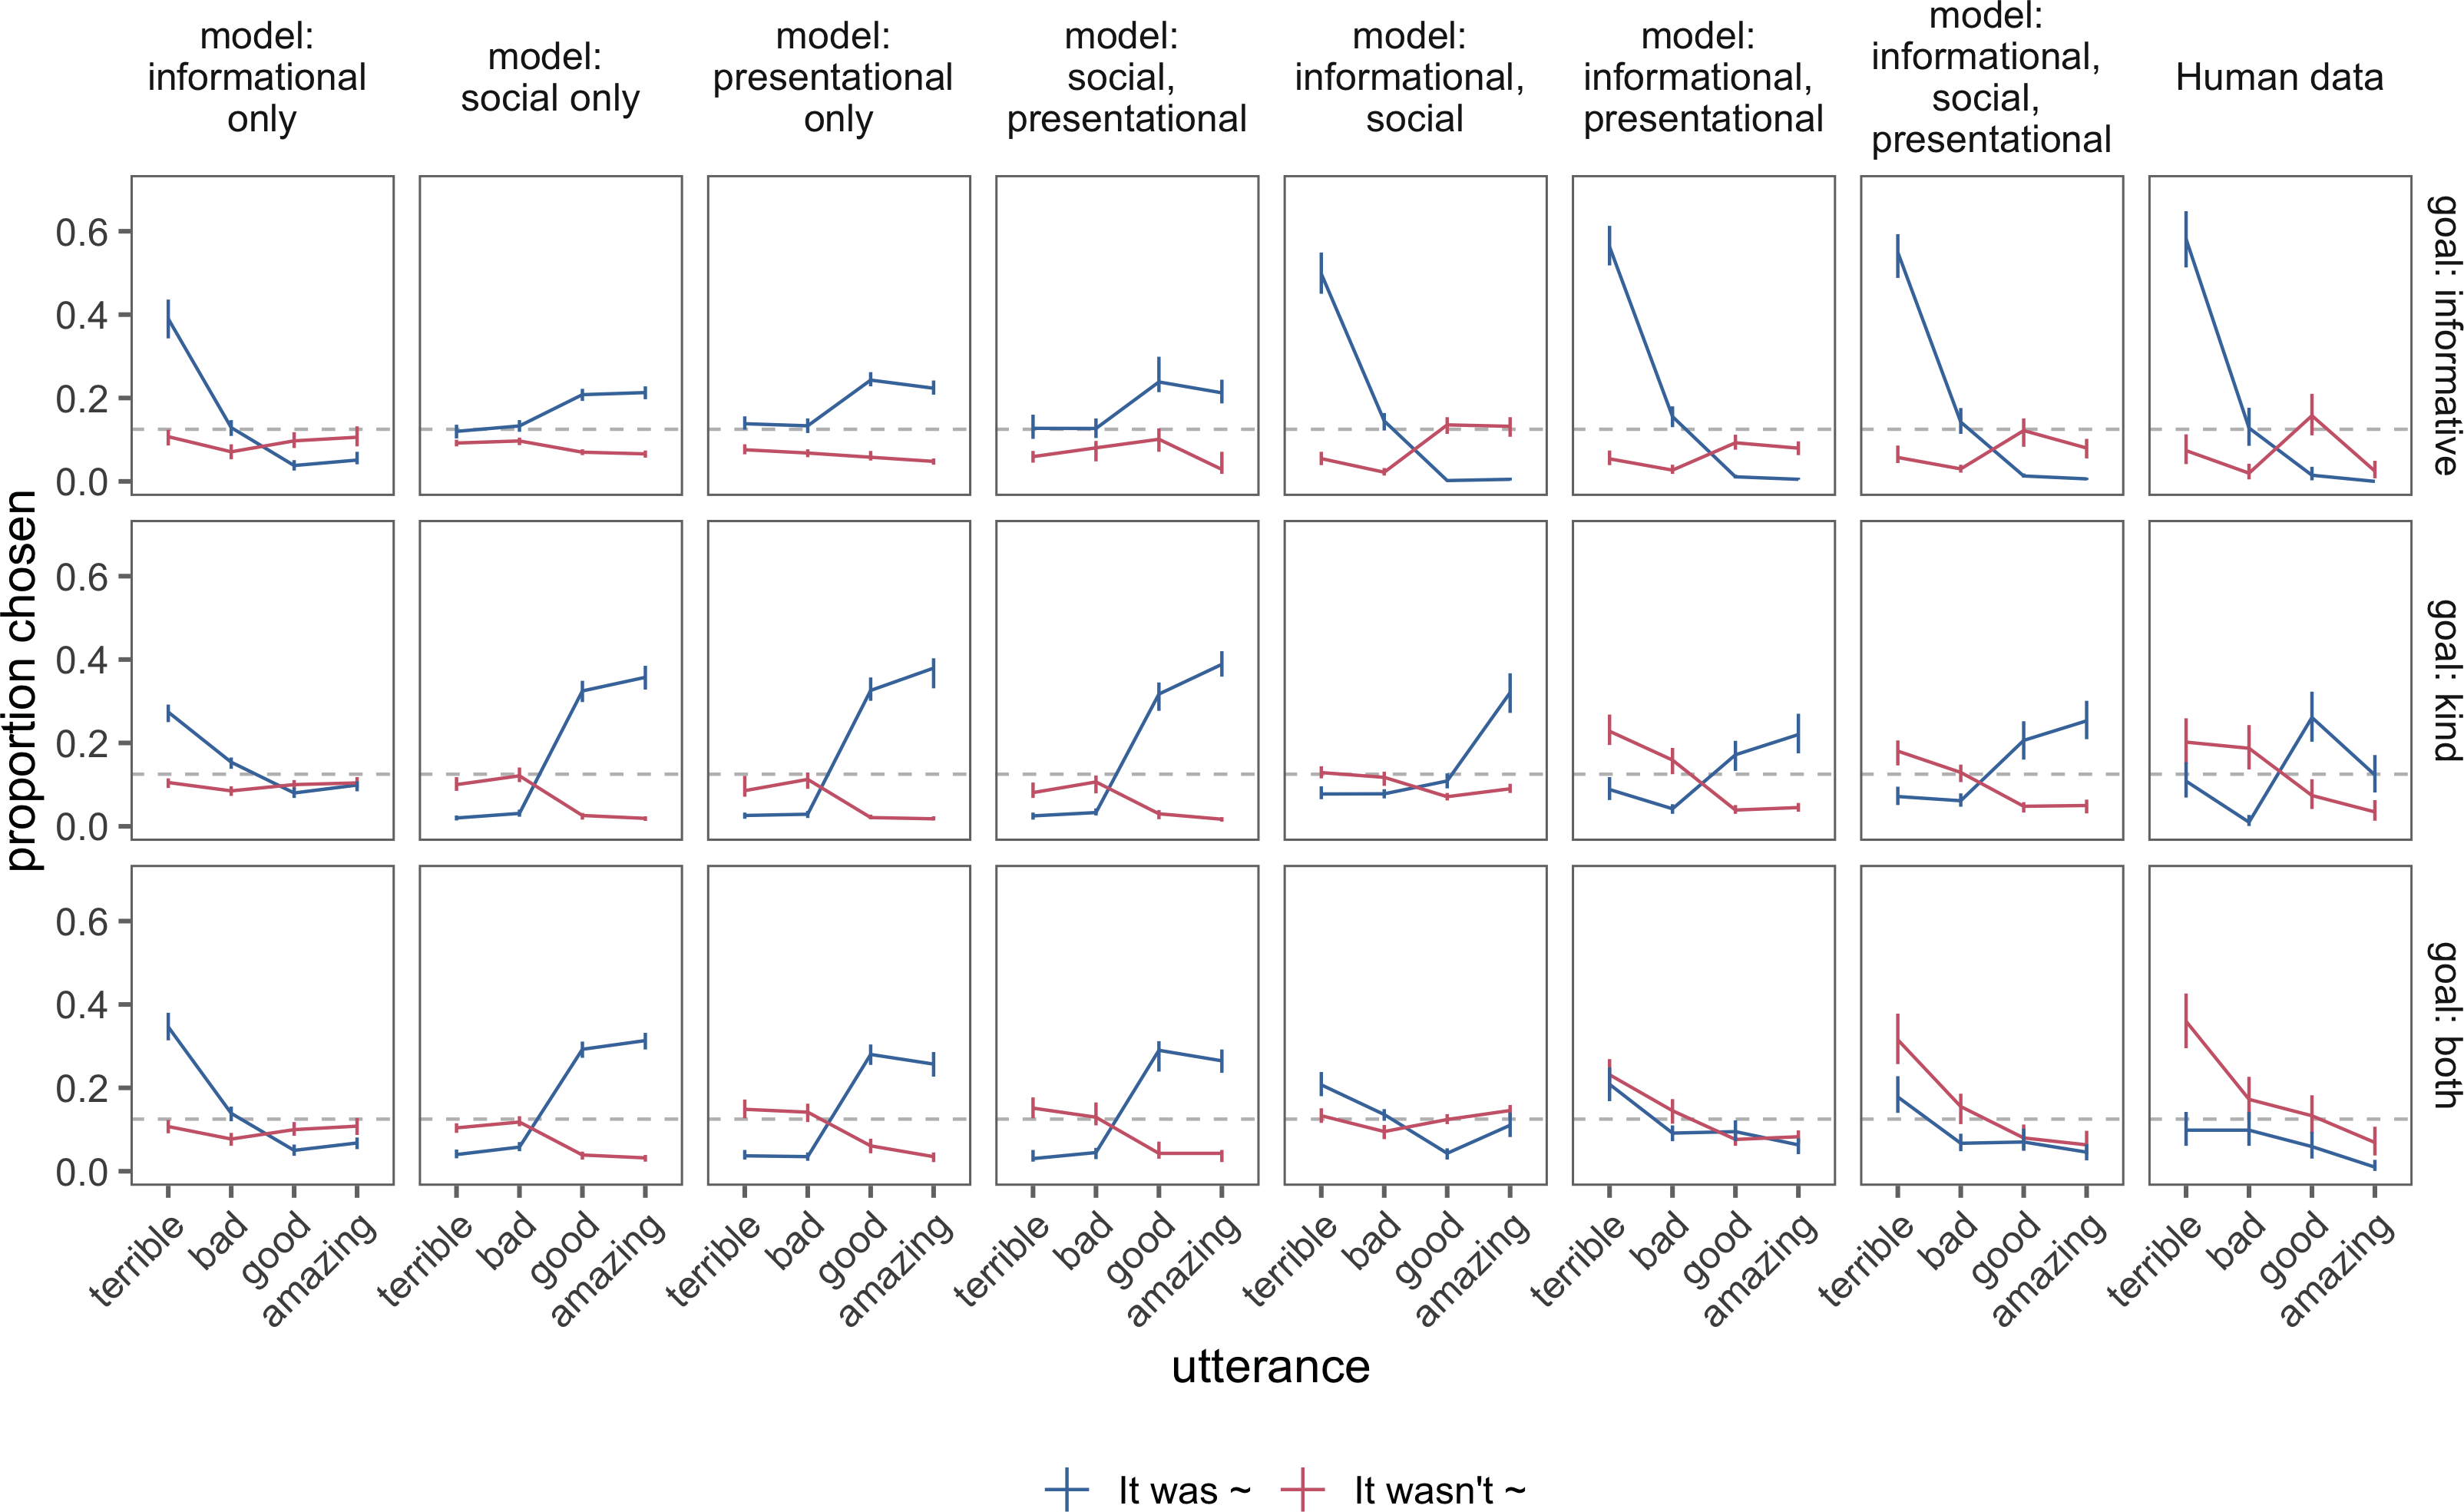
\includegraphics[width=\textwidth]{polite_manuscript_files/figure-latex/comparisonAll-1} \caption{Comparison of predictions for proportion of utterances chosen by pragmatic speaker from possible model variants (left) and human data (rightmost) for average proportion of negation produced among all utterances, given true state of 0 heart and speaker with informative (top), social (middle), and both goals (bottom). Gray dotted line indicates chance level at 12.5\%.}\label{fig:comparisonAll}
\end{figure}

\begin{figure}[!h]
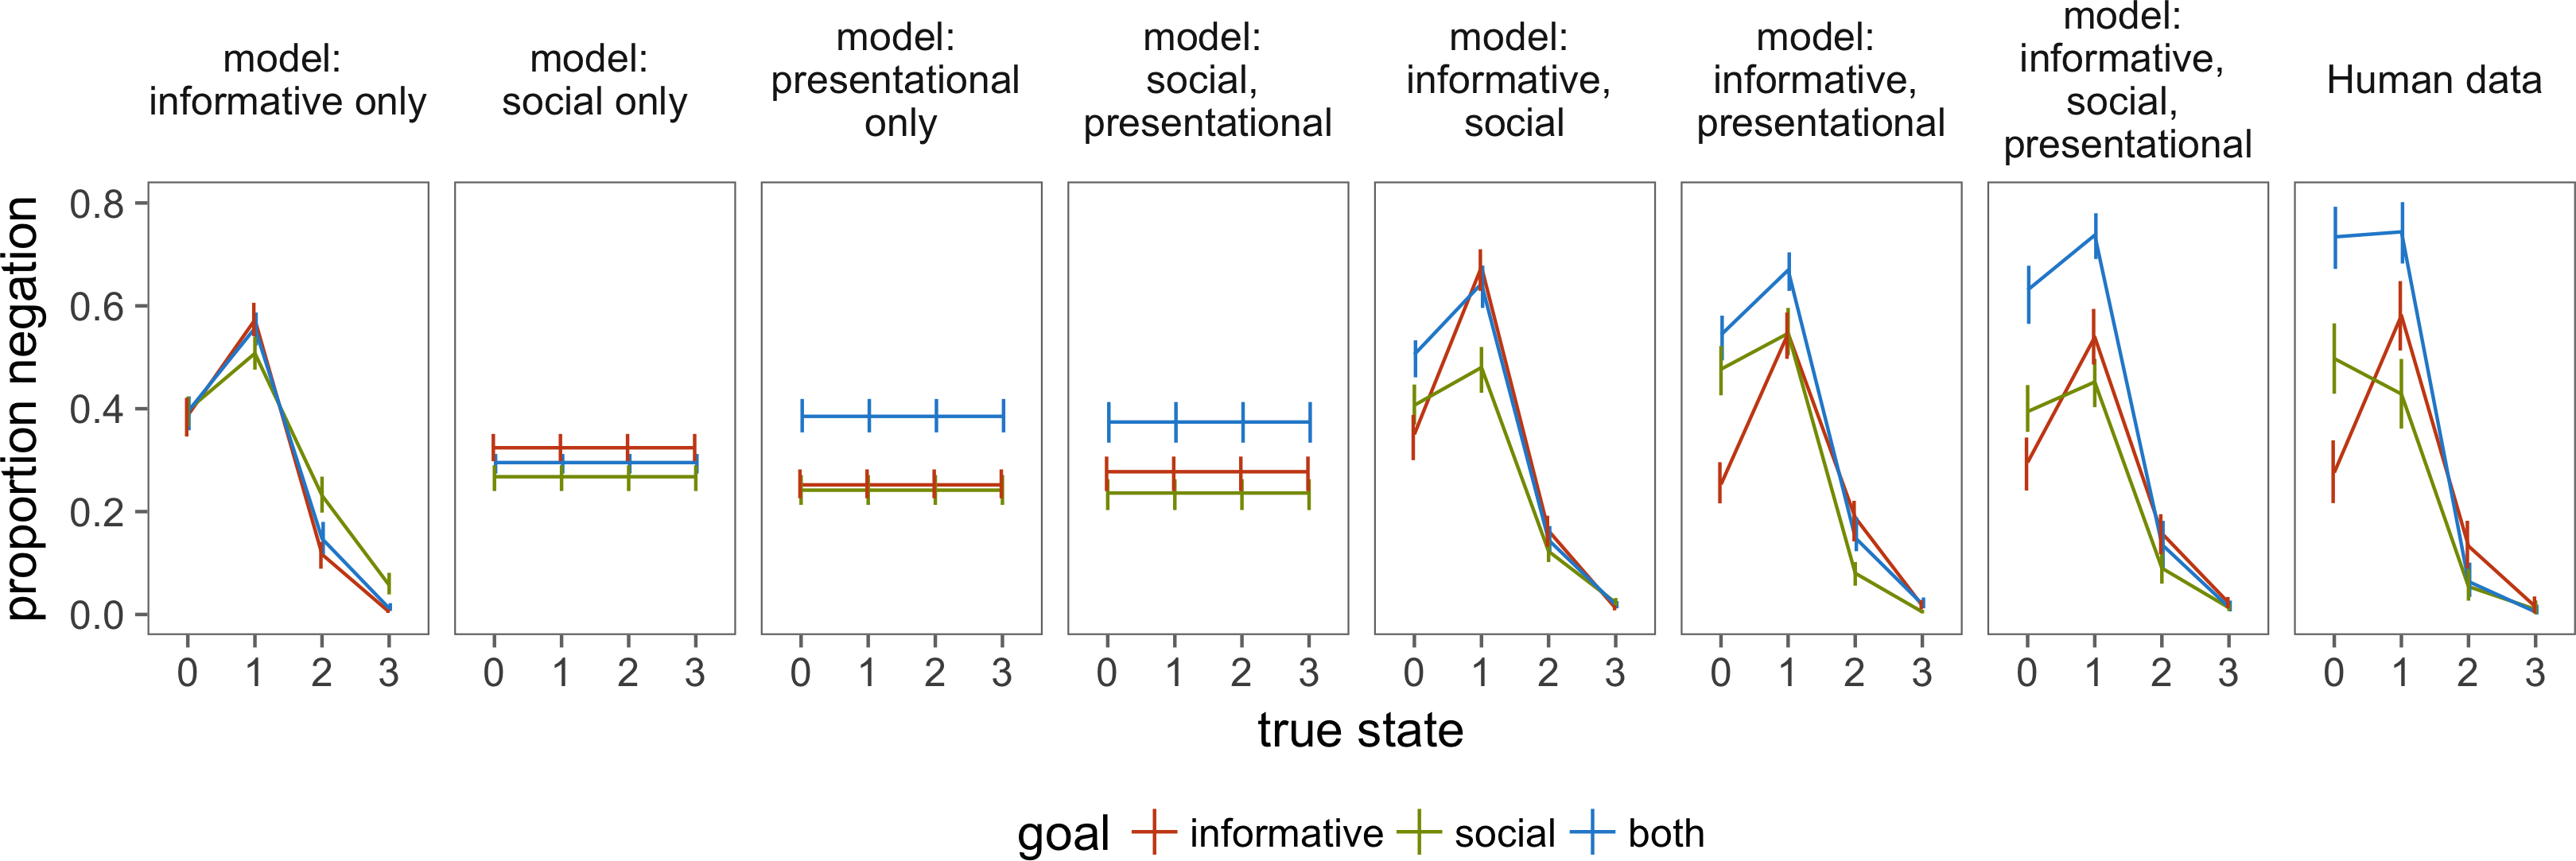
\includegraphics[width=\textwidth]{polite_manuscript_files/figure-latex/negation-1} \caption{Experimental results (left) and fitted model predictions (right) for average proportion of negation produced among all utterances, given true states (x-axis) and goals (colors).}\label{fig:negation}
\end{figure}

.

\newpage

\newpage

\newpage

\pagebreak

\section{References}\label{references}

\setlength{\parindent}{-0.5in} \setlength{\leftskip}{0.5in}

\hypertarget{refs}{}
\hypertarget{ref-R-ggthemes}{}
Arnold, J. B. (2017). \emph{Ggthemes: Extra themes, scales and geoms for
'ggplot2'}. Retrieved from
\url{https://CRAN.R-project.org/package=ggthemes}

\hypertarget{ref-R-gridExtra}{}
Auguie, B. (2017). \emph{GridExtra: Miscellaneous functions for ``grid''
graphics}. Retrieved from
\url{https://CRAN.R-project.org/package=gridExtra}

\hypertarget{ref-R-papaja}{}
Aust, F., \& Barth, M. (2017). \emph{papaja: Create APA manuscripts with
R Markdown}. Retrieved from \url{https://github.com/crsh/papaja}

\hypertarget{ref-R-magrittr}{}
Bache, S. M., \& Wickham, H. (2014). \emph{Magrittr: A forward-pipe
operator for r}. Retrieved from
\url{https://CRAN.R-project.org/package=magrittr}

\hypertarget{ref-baker2017rational}{}
Baker, C. L., Jara-Ettinger, J., Saxe, R., \& Tenenbaum, J. B. (2017).
Rational quantitative attribution of beliefs, desires and percepts in
human mentalizing. \emph{Nature Human Behaviour}, \emph{1}(4), 0064.

\hypertarget{ref-baker2009action}{}
Baker, C. L., Saxe, R., \& Tenenbaum, J. B. (2009). Action understanding
as inverse planning. \emph{Cognition}, \emph{113}(3), 329--349.

\hypertarget{ref-R-Matrix}{}
Bates, D., \& Maechler, M. (2017). \emph{Matrix: Sparse and dense matrix
classes and methods}. Retrieved from
\url{https://CRAN.R-project.org/package=Matrix}

\hypertarget{ref-R-lme4}{}
Bates, D., Mächler, M., Bolker, B., \& Walker, S. (2015). Fitting linear
mixed-effects models using lme4. \emph{Journal of Statistical Software},
\emph{67}(1), 1--48.
doi:\href{https://doi.org/10.18637/jss.v067.i01}{10.18637/jss.v067.i01}

\hypertarget{ref-R-rwebppl}{}
Braginsky, M., Tessler, M. H., \& Hawkins, R. (n.d.). \emph{Rwebppl: R
interface to webppl}. Retrieved from
\url{https://github.com/mhtess/rwebppl}

\hypertarget{ref-R-langcog}{}
Braginsky, M., Yurovsky, D., \& Frank, M. (n.d.). \emph{Langcog:
Language and cognition lab things}. Retrieved from
\url{http://github.com/langcog/langcog}

\hypertarget{ref-brown1987}{}
Brown, P., \& Levinson, S. C. (1987). \emph{Politeness: Some universals
in language usage} (Vol. 4). Cambridge university press.

\hypertarget{ref-buhler1934}{}
Bühler, K. (1934). \emph{Sprachtheorie}. Oxford, England: Fischer.

\hypertarget{ref-R-brms}{}
Bürkner, P.-C. (2017). brms: An R package for bayesian multilevel models
using Stan. \emph{Journal of Statistical Software}, \emph{80}(1), 1--28.
doi:\href{https://doi.org/10.18637/jss.v080.i01}{10.18637/jss.v080.i01}

\hypertarget{ref-R-binom}{}
Dorai-Raj, S. (2014). \emph{Binom: Binomial confidence intervals for
several parameterizations}. Retrieved from
\url{https://CRAN.R-project.org/package=binom}

\hypertarget{ref-R-Rcpp_b}{}
Eddelbuettel, D., \& Balamuta, J. J. (2017). Extending extitR with
extitC++: A Brief Introduction to extitRcpp. \emph{PeerJ Preprints},
\emph{5}, e3188v1.
doi:\href{https://doi.org/10.7287/peerj.preprints.3188v1}{10.7287/peerj.preprints.3188v1}

\hypertarget{ref-R-Rcpp_a}{}
Eddelbuettel, D., \& François, R. (2011). Rcpp: Seamless R and C++
integration. \emph{Journal of Statistical Software}, \emph{40}(8),
1--18.
doi:\href{https://doi.org/10.18637/jss.v040.i08}{10.18637/jss.v040.i08}

\hypertarget{ref-frank2012}{}
Frank, M. C., \& Goodman, N. D. (2012). Predicting pragmatic reasoning
in language games. \emph{Science}, \emph{336}(6084), 998--998.

\hypertarget{ref-goffman1967}{}
Goffman, E. (1967). \emph{Interaction ritual: Essays on face-to-face
interaction}. Aldine.

\hypertarget{ref-goodman2016}{}
Goodman, N. D., \& Frank, M. C. (2016). Pragmatic language
interpretation as probabilistic inference. \emph{Trends in Cognitive
Sciences}, \emph{20}(11), 818--829.

\hypertarget{ref-goodman2013}{}
Goodman, N. D., \& Stuhlmüller, A. (2013). Knowledge and implicature:
Modeling language understanding as social cognition. \emph{Topics in
Cognitive Science}, \emph{5}(1), 173--184.

\hypertarget{ref-grice1975}{}
Grice, H. P. (1975). Logic and conversation. In P. Cole \& J. L. Morgan
(Eds.), \emph{Syntax and semantics} (Vol. 3, pp. 41--58). Academic
Press.

\hypertarget{ref-hamlin2013mentalistic}{}
Hamlin, K. J., Ullman, T. D., Tenenbaum, J. B., Goodman, N. D., \&
Baker, C. L. (2013). The mentalistic basis of core social cognition:
Experiments in preverbal infants and a computational model.
\emph{Developmental Science}, \emph{16}(2), 209--226.

\hypertarget{ref-R-purrr}{}
Henry, L., \& Wickham, H. (2017). \emph{Purrr: Functional programming
tools}. Retrieved from \url{https://CRAN.R-project.org/package=purrr}

\hypertarget{ref-R-directlabels}{}
Hocking, T. D. (2017). \emph{Directlabels: Direct labels for multicolor
plots}. Retrieved from
\url{https://CRAN.R-project.org/package=directlabels}

\hypertarget{ref-ide1989}{}
Ide, S. (1989). Formal forms and discernment: Two neglected aspects of
universals of linguistic politeness. \emph{Multilingua-Journal of
Cross-Cultural and Interlanguage Communication}, \emph{8}(2-3),
223--248.

\hypertarget{ref-jakobson1960}{}
Jakobson, R. (1960). Linguistics and poetics. In \emph{Style in
language} (pp. 350--377). MA: MIT Press.

\hypertarget{ref-jara2016naive}{}
Jara-Ettinger, J., Gweon, H., Schulz, L. E., \& Tenenbaum, J. B. (2016).
The naïve utility calculus: Computational principles underlying
commonsense psychology. \emph{Trends in Cognitive Sciences},
\emph{20}(8), 589--604.

\hypertarget{ref-kao2015}{}
Kao, J. T., \& Goodman, N. D. (2015). Let's talk (ironically) about the
weather: Modeling verbal irony. In \emph{Proceedings of the 37th annual
conference of the Cognitive Science Society}.

\hypertarget{ref-kao2014}{}
Kao, J. T., Wu, J. Y., Bergen, L., \& Goodman, N. D. (2014). Nonliteral
understanding of number words. \emph{Proceedings of the National Academy
of Sciences}, \emph{111}(33), 12002--12007.

\hypertarget{ref-lassiter2017adjectival}{}
Lassiter, D., \& Goodman, N. D. (2017). Adjectival vagueness in a
bayesian model of interpretation. \emph{Synthese}, \emph{194}(10),
3801--3836.

\hypertarget{ref-lee2014}{}
Lee, M. D., \& Wagenmakers, E. J. (2014). \emph{Bayesian cognitive
modeling: A practical course}. Cambridge Univ. Press.

\hypertarget{ref-leech1983}{}
Leech, G. (1983). \emph{Principles of pragmatics}. London, New York:
Longman Group Ltd.

\hypertarget{ref-liu2017ten}{}
Liu, S., Ullman, T. D., Tenenbaum, J. B., \& Spelke, E. S. (2017).
Ten-month-old infants infer the value of goals from the costs of
actions. \emph{Science}, \emph{358}(6366), 1038--1041.

\hypertarget{ref-R-BayesFactor}{}
Morey, R. D., \& Rouder, J. N. (2015). \emph{BayesFactor: Computation of
bayes factors for common designs}. Retrieved from
\url{https://CRAN.R-project.org/package=BayesFactor}

\hypertarget{ref-R-bindrcpp}{}
Müller, K. (2017a). \emph{Bindrcpp: An 'rcpp' interface to active
bindings}. Retrieved from
\url{https://CRAN.R-project.org/package=bindrcpp}

\hypertarget{ref-R-here}{}
Müller, K. (2017b). \emph{Here: A simpler way to find your files}.
Retrieved from \url{https://CRAN.R-project.org/package=here}

\hypertarget{ref-R-tibble}{}
Müller, K., \& Wickham, H. (2017). \emph{Tibble: Simple data frames}.
Retrieved from \url{https://CRAN.R-project.org/package=tibble}

\hypertarget{ref-R-RColorBrewer}{}
Neuwirth, E. (2014). \emph{RColorBrewer: ColorBrewer palettes}.
Retrieved from \url{https://CRAN.R-project.org/package=RColorBrewer}

\hypertarget{ref-R-jsonlite}{}
Ooms, J. (2014). The jsonlite package: A practical and consistent
mapping between json data and r objects. \emph{arXiv:1403.2805
{[}Stat.CO{]}}. Retrieved from \url{https://arxiv.org/abs/1403.2805}

\hypertarget{ref-R-coda}{}
Plummer, M., Best, N., Cowles, K., \& Vines, K. (2006). CODA:
Convergence diagnosis and output analysis for mcmc. \emph{R News},
\emph{6}(1), 7--11. Retrieved from
\url{https://journal.r-project.org/archive/}

\hypertarget{ref-R-base}{}
R Core Team. (2017). \emph{R: A language and environment for statistical
computing}. Vienna, Austria: R Foundation for Statistical Computing.
Retrieved from \url{https://www.R-project.org/}

\hypertarget{ref-searle1975}{}
Searle, J. (1975). Indirect speech acts. In P. Cole \& J. L. Morgan
(Eds.), \emph{Syntax and semantics} (Vol. 3, pp. 59--82). Academic
Press.

\hypertarget{ref-shannon1948}{}
Shannon, C. E. (1948). A mathematical theory of communication.
\emph{Bell Syst. Tech. J.}, \emph{27}, 623--656.

\hypertarget{ref-R-ggplot2}{}
Wickham, H. (2009). \emph{Ggplot2: Elegant graphics for data analysis}.
Springer-Verlag New York. Retrieved from \url{http://ggplot2.org}

\hypertarget{ref-R-forcats}{}
Wickham, H. (2017a). \emph{Forcats: Tools for working with categorical
variables (factors)}. Retrieved from
\url{https://CRAN.R-project.org/package=forcats}

\hypertarget{ref-R-stringr}{}
Wickham, H. (2017b). \emph{Stringr: Simple, consistent wrappers for
common string operations}. Retrieved from
\url{https://CRAN.R-project.org/package=stringr}

\hypertarget{ref-R-tidyverse}{}
Wickham, H. (2017c). \emph{Tidyverse: Easily install and load the
'tidyverse'}. Retrieved from
\url{https://CRAN.R-project.org/package=tidyverse}

\hypertarget{ref-R-tidyr}{}
Wickham, H., \& Henry, L. (2017). \emph{Tidyr: Easily tidy data with
'spread()' and 'gather()' functions}. Retrieved from
\url{https://CRAN.R-project.org/package=tidyr}

\hypertarget{ref-R-dplyr}{}
Wickham, H., Francois, R., Henry, L., \& Müller, K. (2017). \emph{Dplyr:
A grammar of data manipulation}. Retrieved from
\url{https://CRAN.R-project.org/package=dplyr}

\hypertarget{ref-R-readr}{}
Wickham, H., Hester, J., \& Francois, R. (2017). \emph{Readr: Read
rectangular text data}. Retrieved from
\url{https://CRAN.R-project.org/package=readr}






\end{document}
